\documentclass[11pt]{article}
\usepackage[margin=1in]{geometry}
\usepackage{amsmath,amssymb}
\usepackage{graphicx}
\usepackage{booktabs}
\usepackage{enumitem}
\usepackage{xcolor}
\usepackage{listings}
\usepackage{float}
\usepackage{hyperref}

\lstset{basicstyle=\ttfamily\scriptsize, keywordstyle=\color{blue!70!black},
        stringstyle=\color{red!60!black}, language=Python, frame=single, breaklines=true, numbers=left,
        numberstyle=\tiny\color{gray}, columns=fullflexible, showstringspaces=false}

\title{EECE 5639: Computer Vision\\Fall 2026, Homework 2}
\author{Jingqi Mei}
\date{October 9, 2026}

\setlength{\emergencystretch}{3em}
\begin{document}
\maketitle

%=====================================================================
\section*{Problem 1}
%=====================================================================
$I_k = \hat I_k + N_k$, \; $N_k \sim \mathcal N(0,\sigma^2)$ i.i.d., \;
$I_i^{\text{out}} = w_1 I_{i-1} + w_2 I_i + w_3 I_{i+1}$, \; $w_1+w_2+w_3=1$.

\subsection*{(a)}
\[
I_i^{\text{out}} = \left(w_1\hat I_{i-1} + w_2\hat I_i + w_3\hat I_{i+1}\right) + \left(w_1N_{i-1} + w_2N_i + w_3N_{i+1}\right)
\]
\[
\boxed{N_i^{\text{out}} = w_1N_{i-1} + w_2N_i + w_3N_{i+1}}
\]

\subsection*{(b)}
The noise has zero mean and is independent, so all cross terms $E[N_jN_k]$, $j\neq k$, vanish:
\[
\boxed{\operatorname{Var}(N_i^{\text{out}}) = \sigma^2\left(w_1^2+w_2^2+w_3^2\right)}
\]

\subsection*{(c)}
\[
L(w_1,w_2,w_3;\lambda) = \sigma^2\left(w_1^2+w_2^2+w_3^2\right) + \lambda\left(w_1+w_2+w_3-1\right)
\]
\[
\frac{\partial L}{\partial w_k} = 2\sigma^2 w_k + \lambda = 0 \;\Rightarrow\; w_k = -\frac{\lambda}{2\sigma^2}\quad (k=1,2,3),
\qquad
\frac{\partial L}{\partial \lambda} = w_1+w_2+w_3-1 = 0.
\]
Hence $w_1=w_2=w_3$, and the constraint gives $3\left(-\frac{\lambda}{2\sigma^2}\right)=1$, so $\lambda^*=-\frac{2\sigma^2}{3}$ and
\[
\boxed{w_1^* = w_2^* = w_3^* = \tfrac13}
\]
This is the minimum: the objective is strictly convex (Hessian $2\sigma^2\mathbf I \succ 0$) and the constraint is linear.

\subsection*{(d)}
The \textbf{box (mean) filter} $\left[\tfrac13\;\tfrac13\;\tfrac13\right]$.

\subsection*{(e)}
$\sigma^2_{\text{out}} = 3\cdot\tfrac19\sigma^2 = \sigma^2/3$, so the noise variance is reduced by a \textbf{factor of 3}.

\subsection*{(f)}
The box weights all neighbours equally, so pixels on the other side of an edge count as much as the centre pixel. Edges become blurred ramps, and thin lines and fine details lose contrast. Its sinc-shaped frequency response also has sidelobes, which cause ringing and blocky artifacts. A Gaussian puts most of the weight on the nearest pixels, so it keeps edges and details sharper. It has a smooth frequency response with no ringing, and its smoothing strength can be tuned with $\sigma$. It removes slightly less noise than the box but usually gives a better-looking image.

%=====================================================================
\section*{Problem 2}
%=====================================================================
Code: \texttt{hw2\_q2.py} (Appendix). The image is normalized to $[0,1]$. Panel titles show the PSNR with respect to the clean image.

\subsection*{(a)}
\begin{figure}[H]\centering
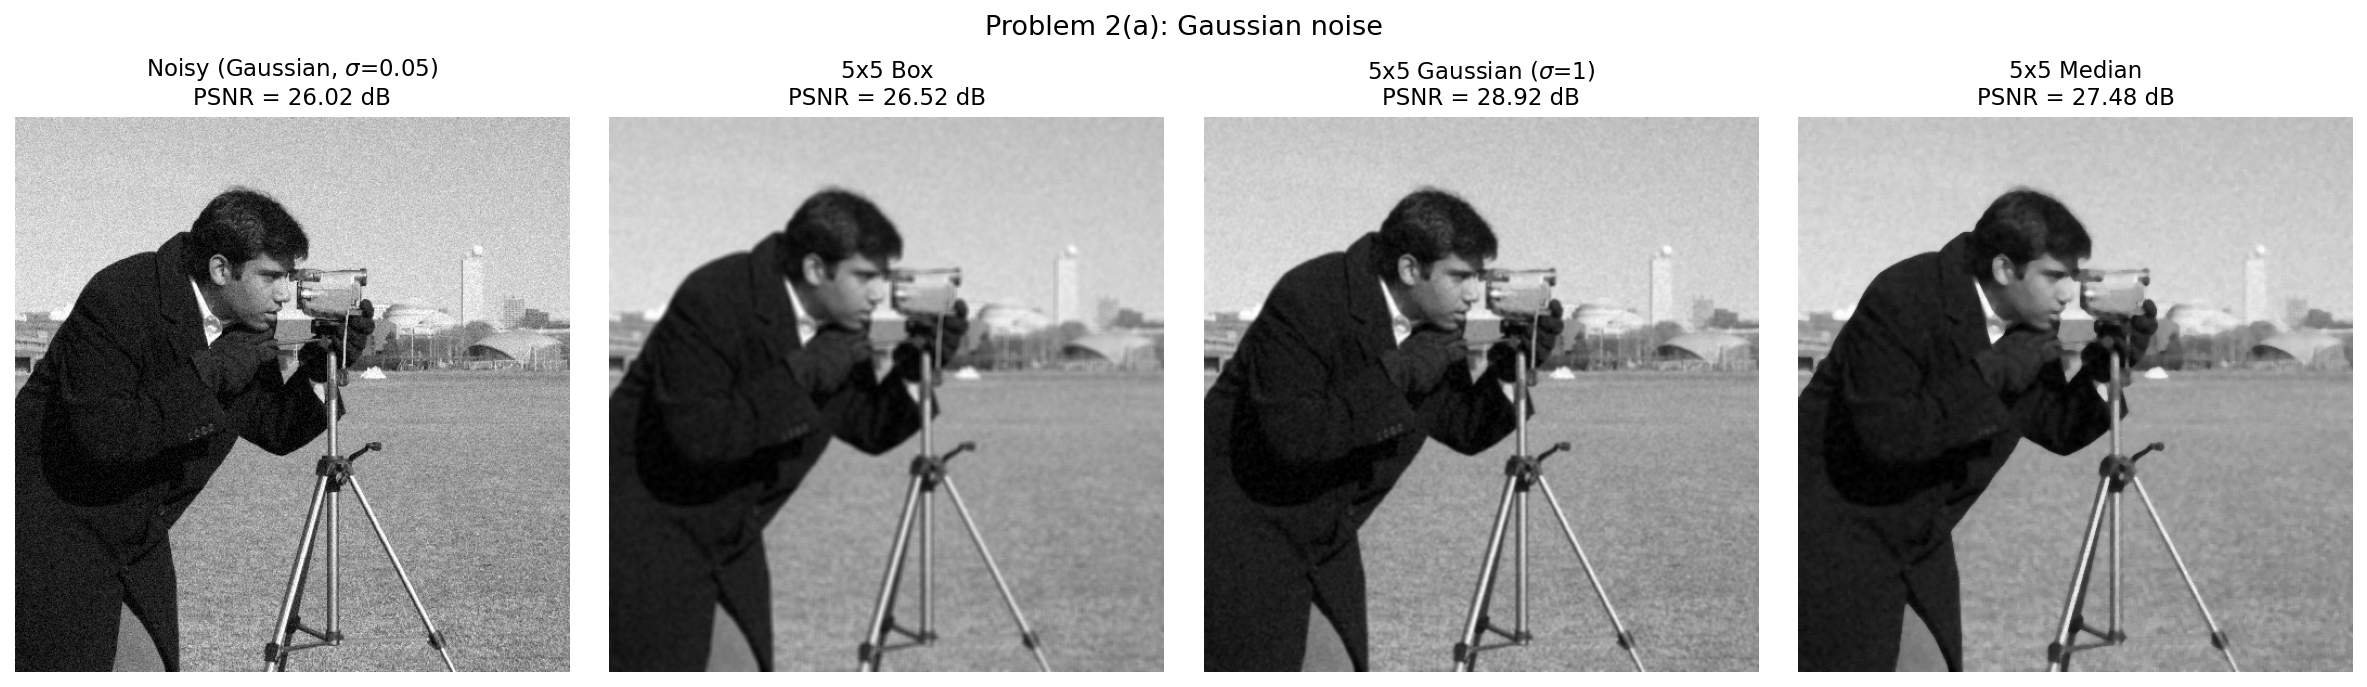
\includegraphics[width=\linewidth]{figures/q2a_gaussian_noise.png}\\[2pt]
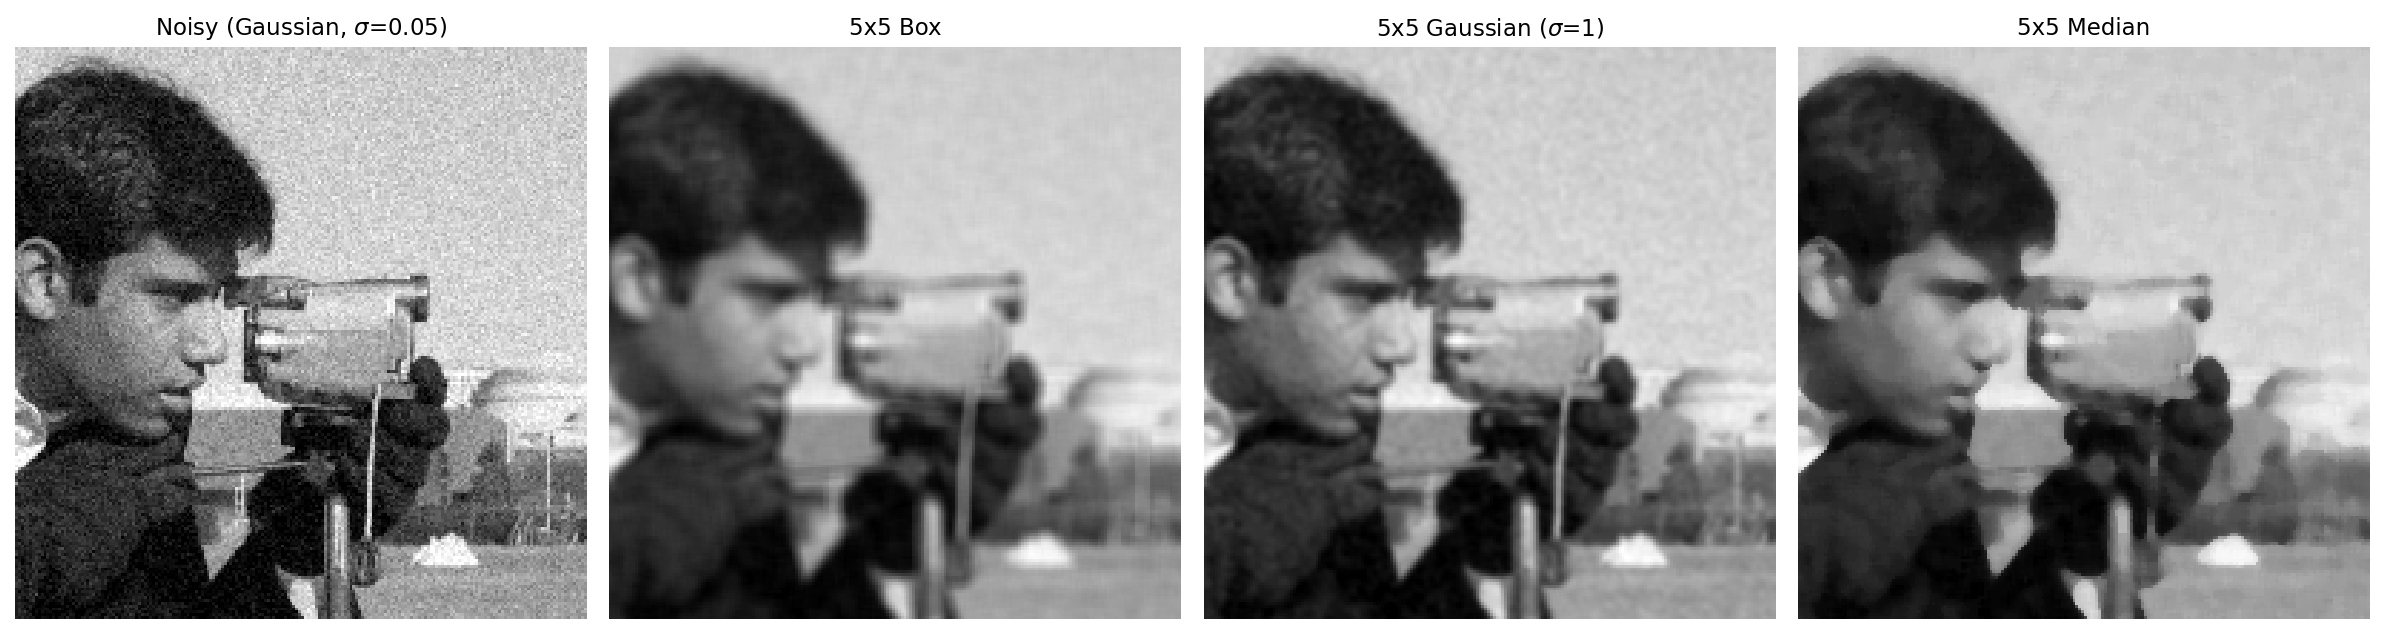
\includegraphics[width=\linewidth]{figures/q2a_zoom.png}
\caption{Gaussian noise ($\sigma=0.05$) and the three $5\times5$ filters (bottom: zoom).}
\end{figure}

\begin{table}[H]\centering\small
\begin{tabular}{lcccc}\toprule
 & Noisy & Box & Gaussian & Median\\\midrule
PSNR (dB) & 26.02 & 26.52 & \textbf{28.92} & 27.48\\
Residual noise std (flat sky) & 0.0499 & \textbf{0.0099} & 0.0142 & 0.0126\\
Edge gradient (clean: 1.04) & 1.043 & 0.442 & \textbf{0.656} & 0.586\\\bottomrule
\end{tabular}
\end{table}

\subsection*{(b)}
\begin{enumerate}[label=\roman*., leftmargin=*]
\item The \textbf{Box filter} removes the most noise. It leaves the lowest residual noise (0.0099), which matches the theoretical $0.05/5$.
\item \textbf{No.} The box image is the blurriest: edges, the face and the tripod are smeared, and it has the lowest PSNR. The \textbf{Gaussian} gives the best-looking image. The median keeps strong edges but makes flat areas look blotchy and removes thin details.
\item The box gives all 25 pixels the same weight (0.04). The Gaussian weights the centre most (0.16) and the corners very little (0.003). The box therefore averages more, removing more noise but causing more blur. The Gaussian averages more locally and keeps more detail.
\end{enumerate}

\subsection*{(c)}
\begin{figure}[H]\centering
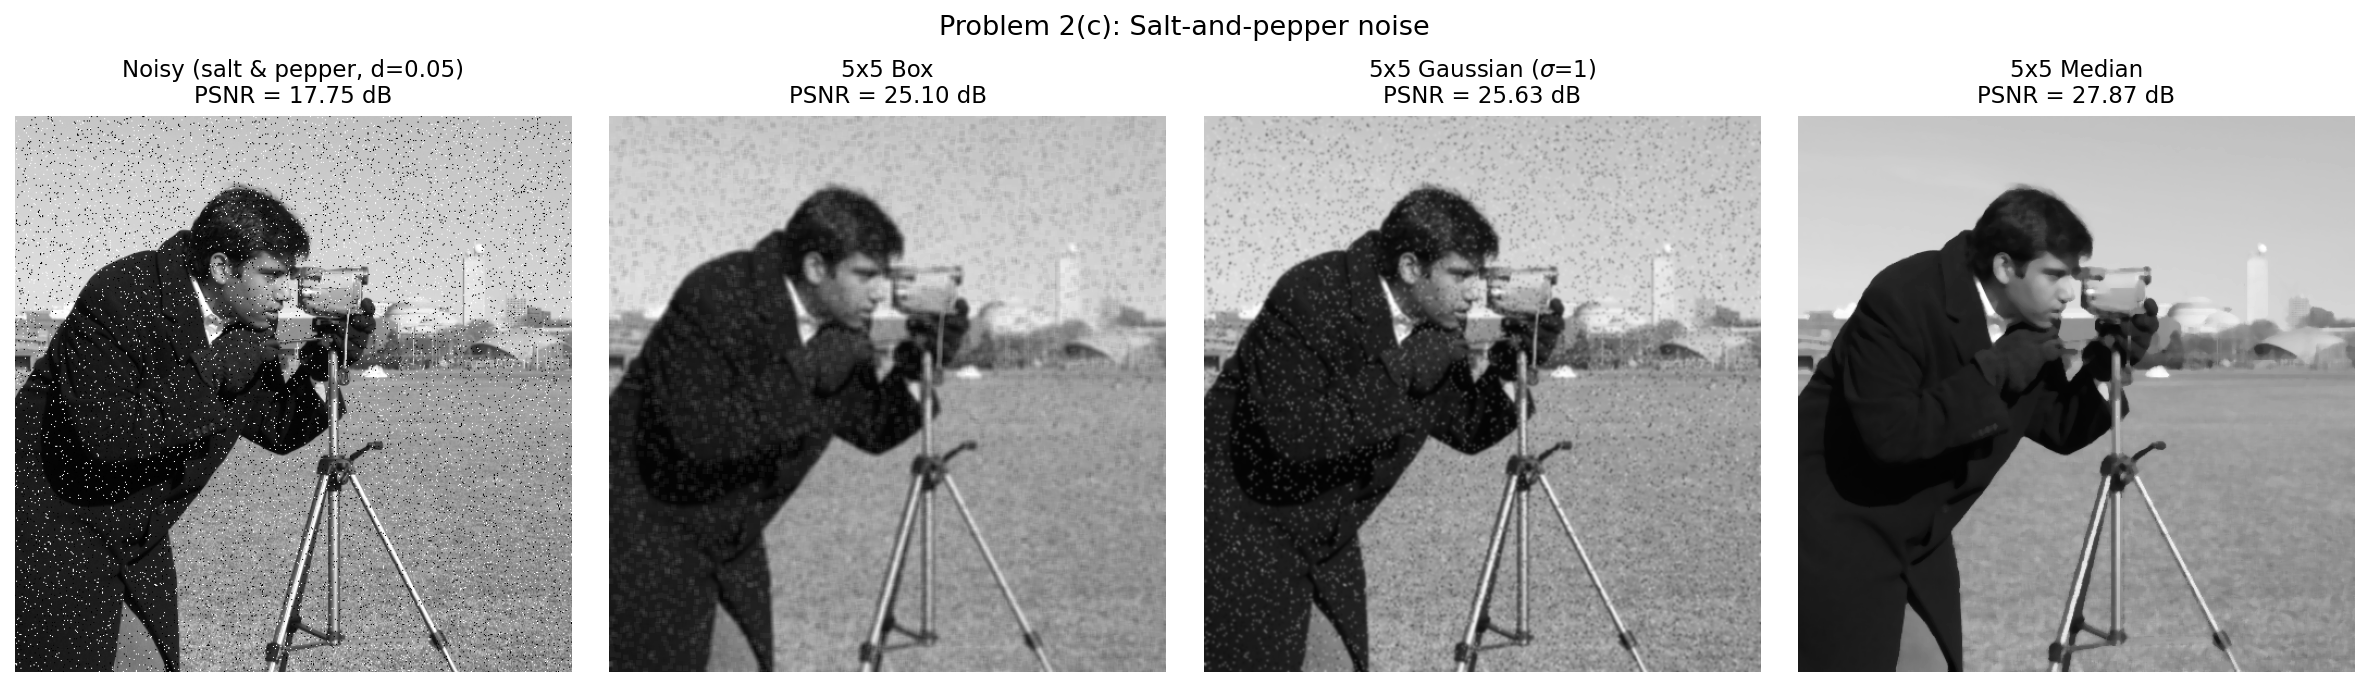
\includegraphics[width=\linewidth]{figures/q2c_salt_pepper.png}\\[2pt]
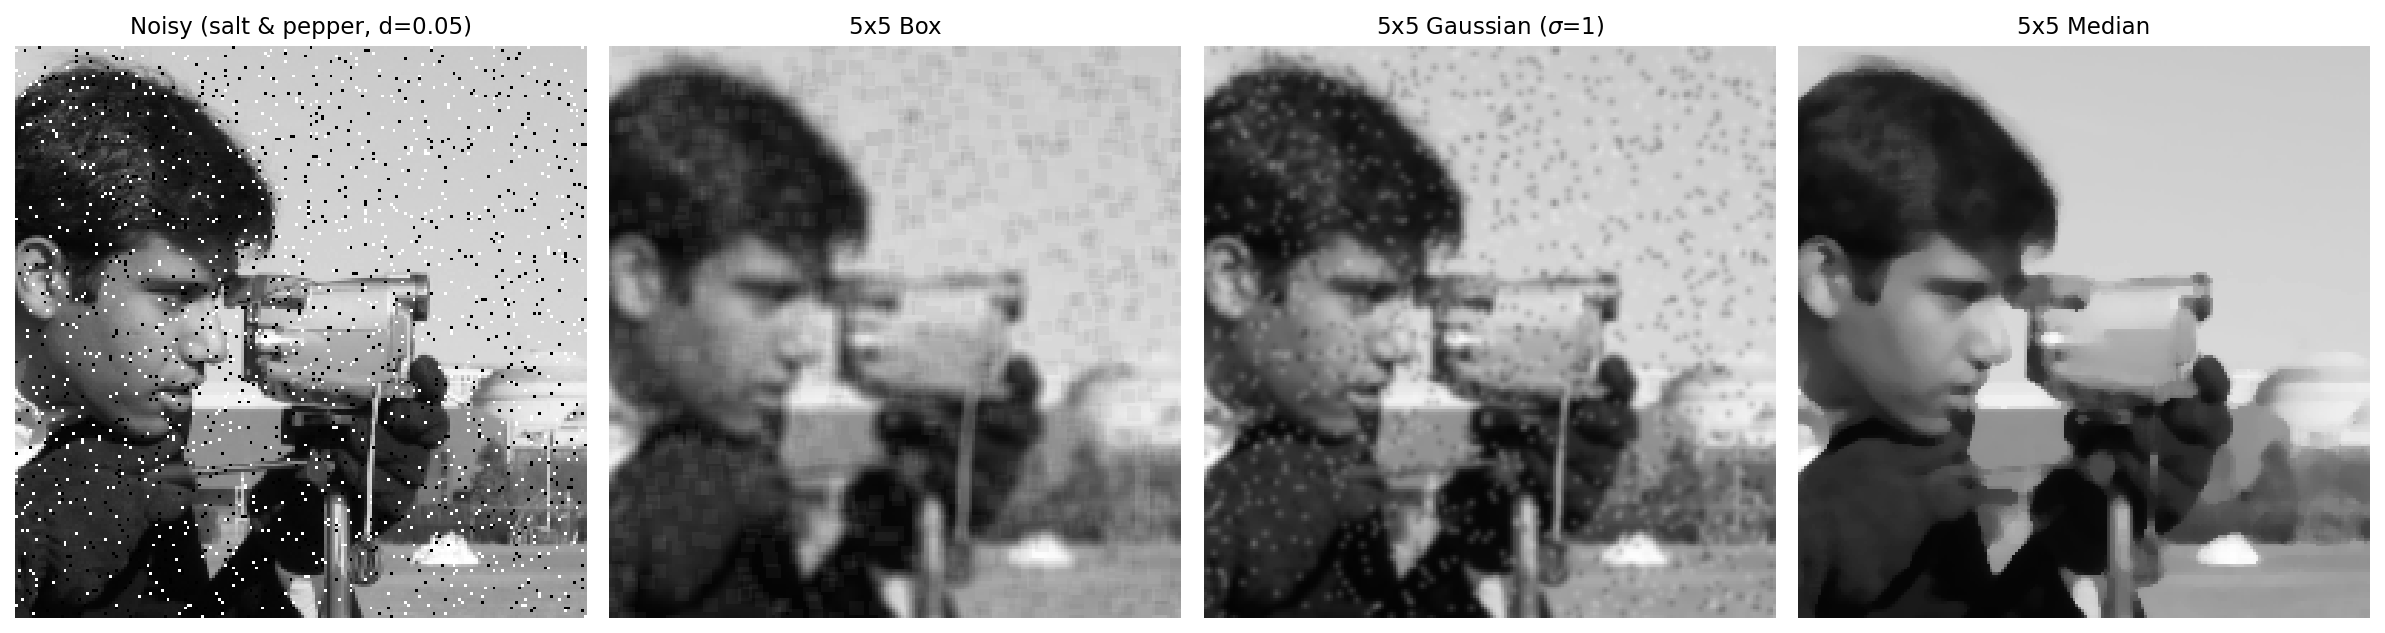
\includegraphics[width=\linewidth]{figures/q2c_zoom.png}
\caption{Salt-and-pepper noise ($d=0.05$) and the three $5\times5$ filters (bottom: zoom).}
\end{figure}

\subsection*{(d)}
\begin{enumerate}[label=\roman*., leftmargin=*]
\item The \textbf{Median filter}: almost all impulses are removed (27.87 dB vs.\ about 25 dB for Box and Gaussian).
\item Salt-and-pepper pixels are outliers. A $5\times5$ window contains only about 1--2 of them, so the median ignores them and outputs the value of a real neighbouring pixel. Linear filters instead spread each impulse into a visible blob.
\item In the Gaussian-noise case the median was only second (27.48 dB vs.\ 28.92 dB for the Gaussian). There every pixel is slightly corrupted and there are no outliers to reject, and the median gives blotchy results. It works best for impulse noise.
\end{enumerate}

\subsection*{(e)}
\begin{figure}[H]\centering
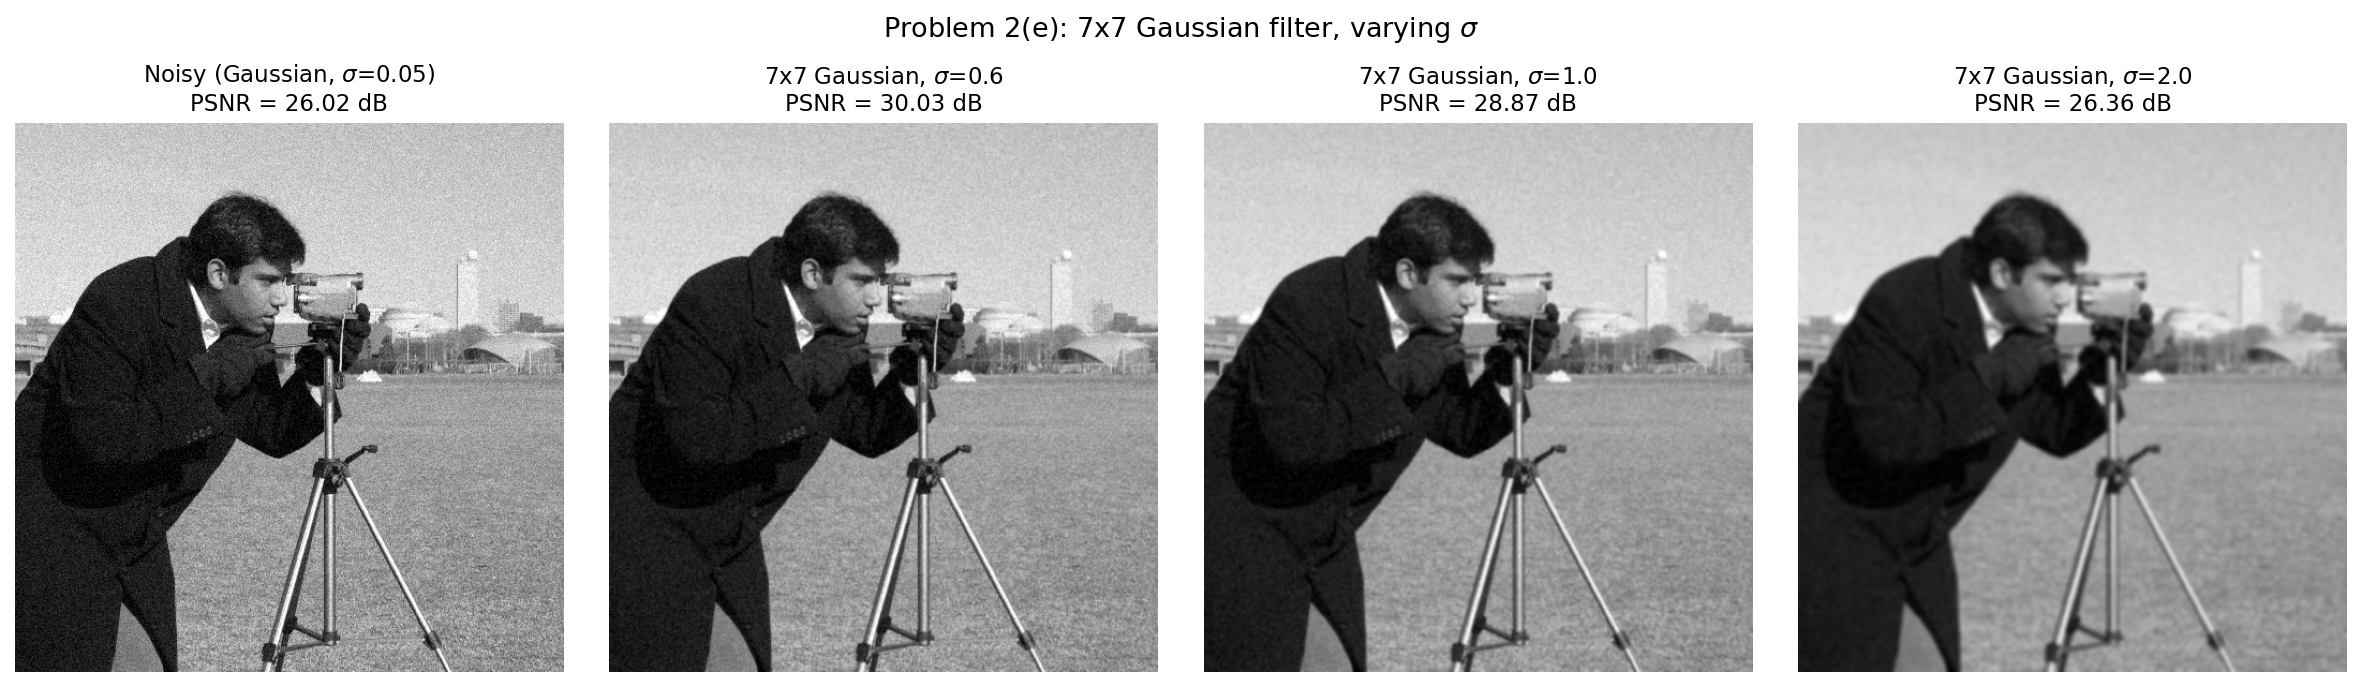
\includegraphics[width=\linewidth]{figures/q2e_gaussian_sigma.png}\\[2pt]
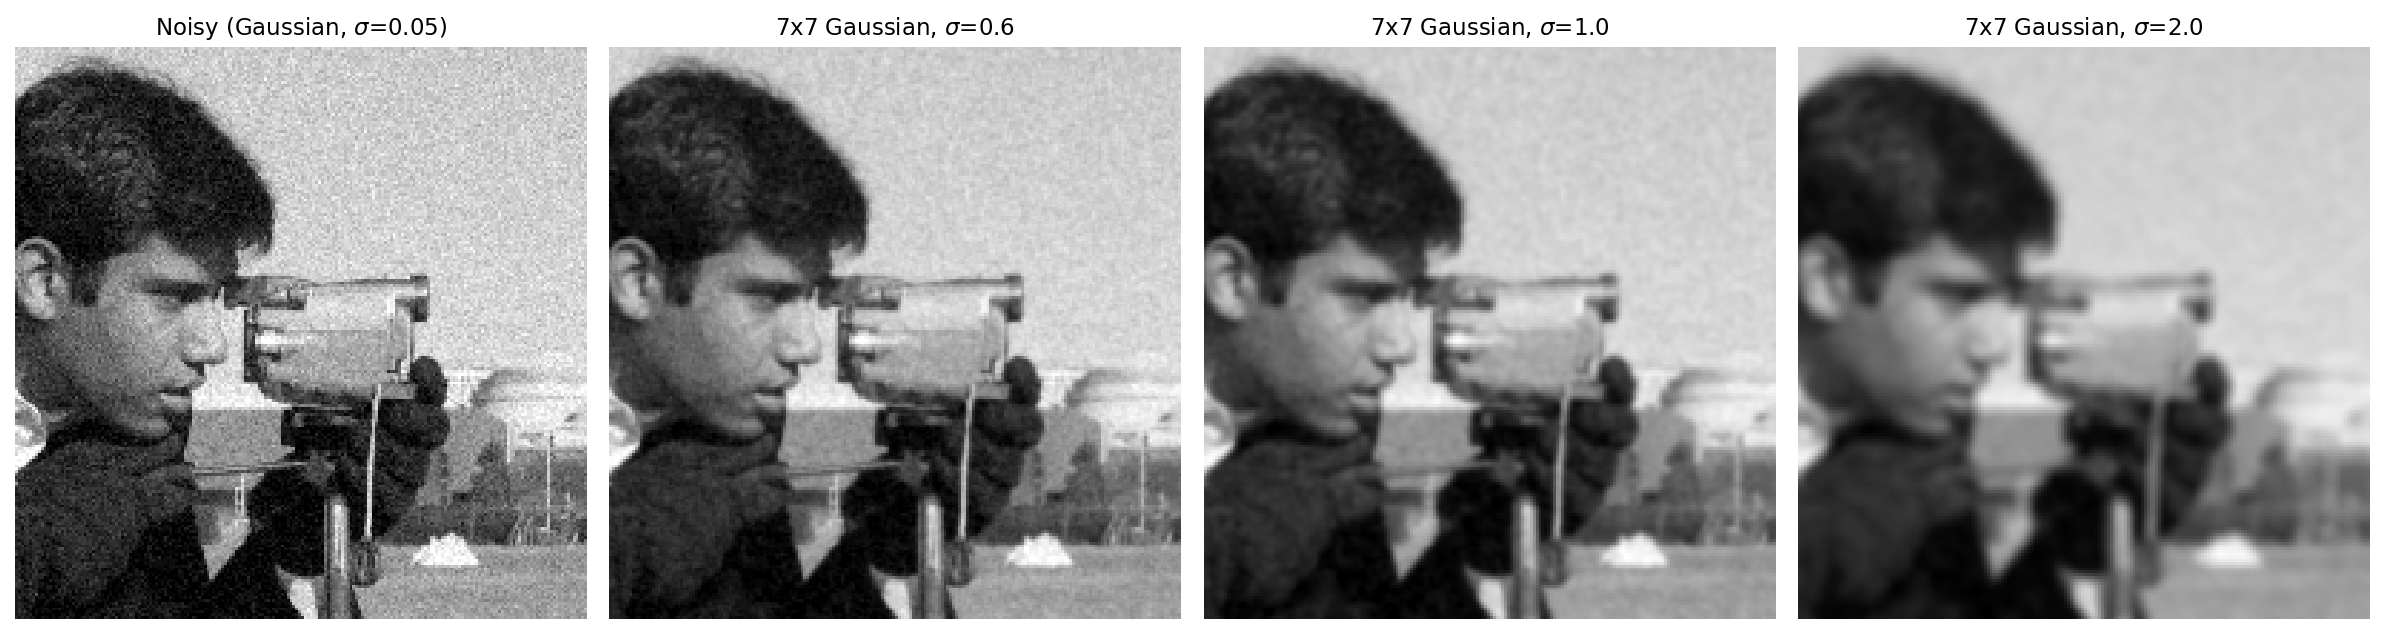
\includegraphics[width=\linewidth]{figures/q2e_zoom.png}
\caption{$7\times7$ Gaussian filter with $\sigma = 0.6, 1, 2$ (bottom: zoom).}
\end{figure}

\begin{table}[H]\centering\small
\begin{tabular}{lccc}\toprule
 & $\sigma=0.6$ & $\sigma=1$ & $\sigma=2$\\\midrule
1-D centre weight & 0.664 & 0.399 & 0.216\\
Residual noise std (flat sky) & 0.0246 & 0.0140 & \textbf{0.0081}\\
Edge gradient (clean: 1.04) & \textbf{0.850} & 0.647 & 0.400\\
PSNR (dB) & \textbf{30.03} & 28.87 & 26.36\\\bottomrule
\end{tabular}
\end{table}

\subsection*{(f)}
As $\sigma$ increases:
\begin{itemize}[leftmargin=*]
\item \textbf{Noise reduction increases}: the residual noise drops from 0.0246 to 0.0081.
\item \textbf{More fine detail is lost}: the hair, the face and the grass texture fade away at $\sigma=2$.
\item \textbf{Edges become less sharp}: the edge gradient drops from 0.85 to 0.40.
\end{itemize}
This is consistent with the kernel weights. A small $\sigma$ concentrates the weight on the centre pixel (0.66), so there is little averaging. A large $\sigma$ spreads the weight almost evenly over the $7\times7$ window, so the filter behaves like a box: more averaging, less noise, more blur.

\subsection*{(g)}
\begin{enumerate}[leftmargin=*]
\item \textbf{Noise type:} for Gaussian noise, which affects every pixel, use a linear filter; the Gaussian is best. For salt-and-pepper noise, which consists of outliers, use the median filter.
\item \textbf{Trade-off:} stronger smoothing (a box, or a Gaussian with large $\sigma$) removes more noise but blurs edges and details. The filter that removes the most noise does not give the best image.
\item \textbf{Choosing $\sigma$:} use the smallest $\sigma$ that removes enough noise. Here $\sigma\approx0.6$--$1$ works well and $\sigma=2$ over-smooths.
\end{enumerate}

%=====================================================================
\section*{Problem 3}
%=====================================================================
Code: \texttt{hw2\_q3.py} (Appendix). Prewitt and Sobel come from \texttt{scipy.ndimage}; Canny is \texttt{skimage.feature.canny} with default settings. Gradient images are scaled to their 99.5th percentile for display.

\subsection*{(a)}
\begin{figure}[H]\centering
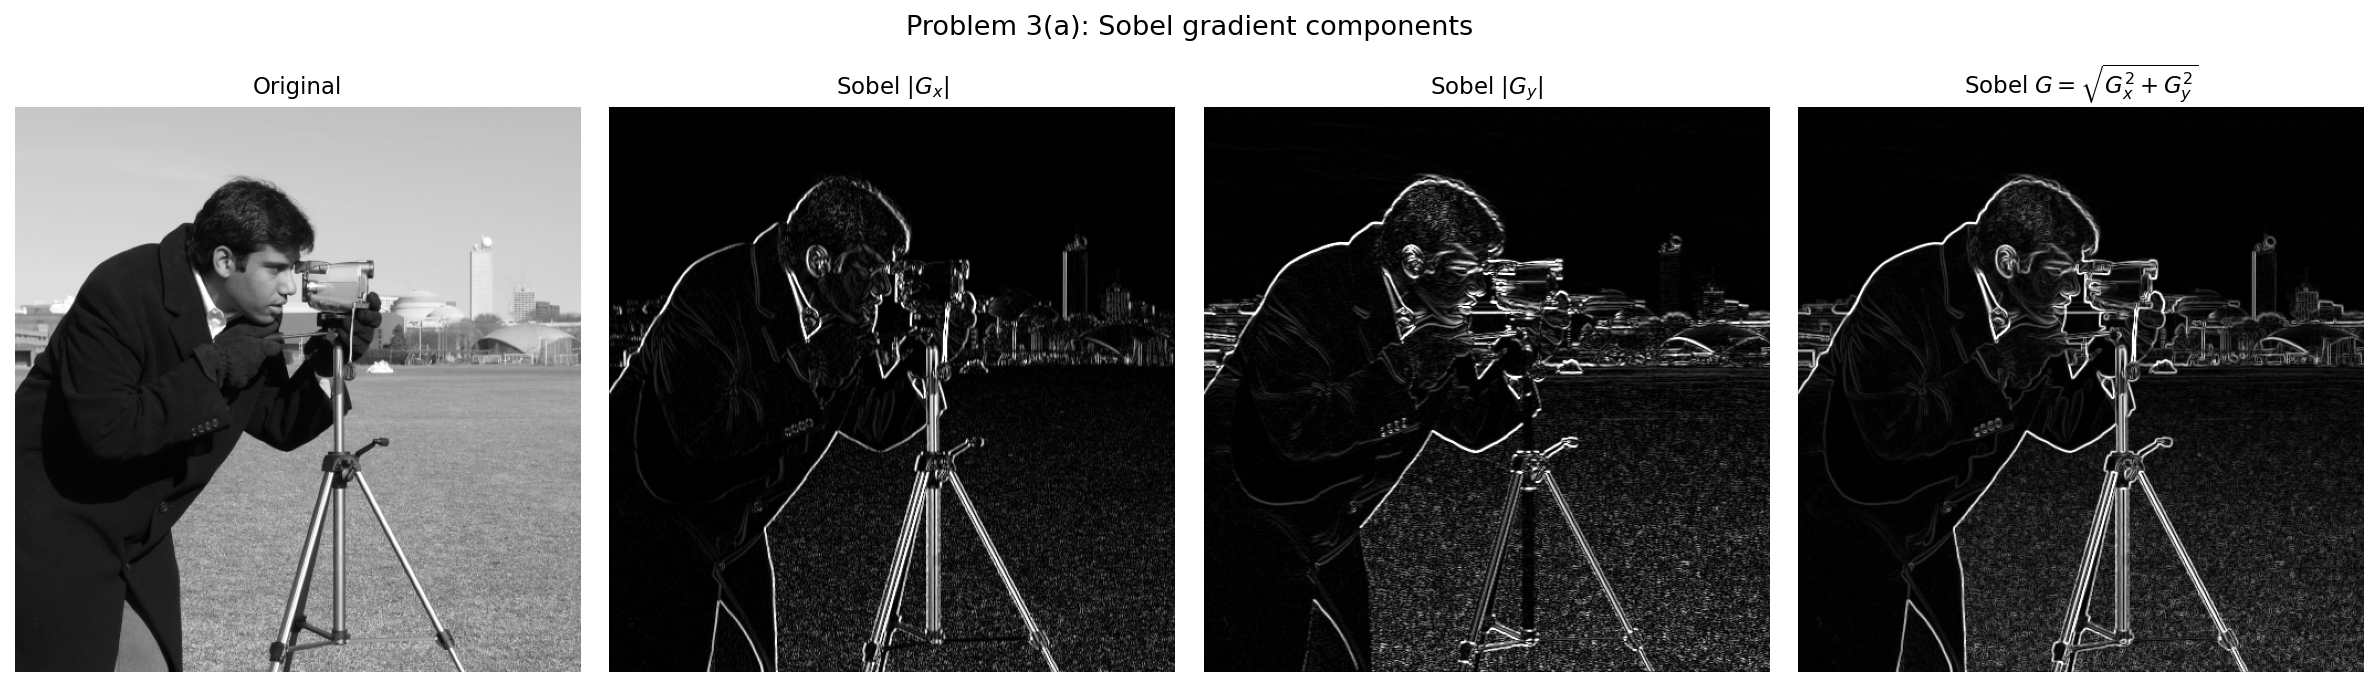
\includegraphics[width=\linewidth]{figures/q3a_sobel_components.png}
\end{figure}
$|G_x|$ responds to horizontal intensity changes, so it highlights \textbf{vertical edges} (the coat outline, the tripod legs, the buildings). $|G_y|$ highlights \textbf{horizontal edges} (the horizon, the top and bottom of the camera, the shoulders). $G$ combines the two, showing edges of all orientations.

\subsection*{(b)}
\begin{figure}[H]\centering
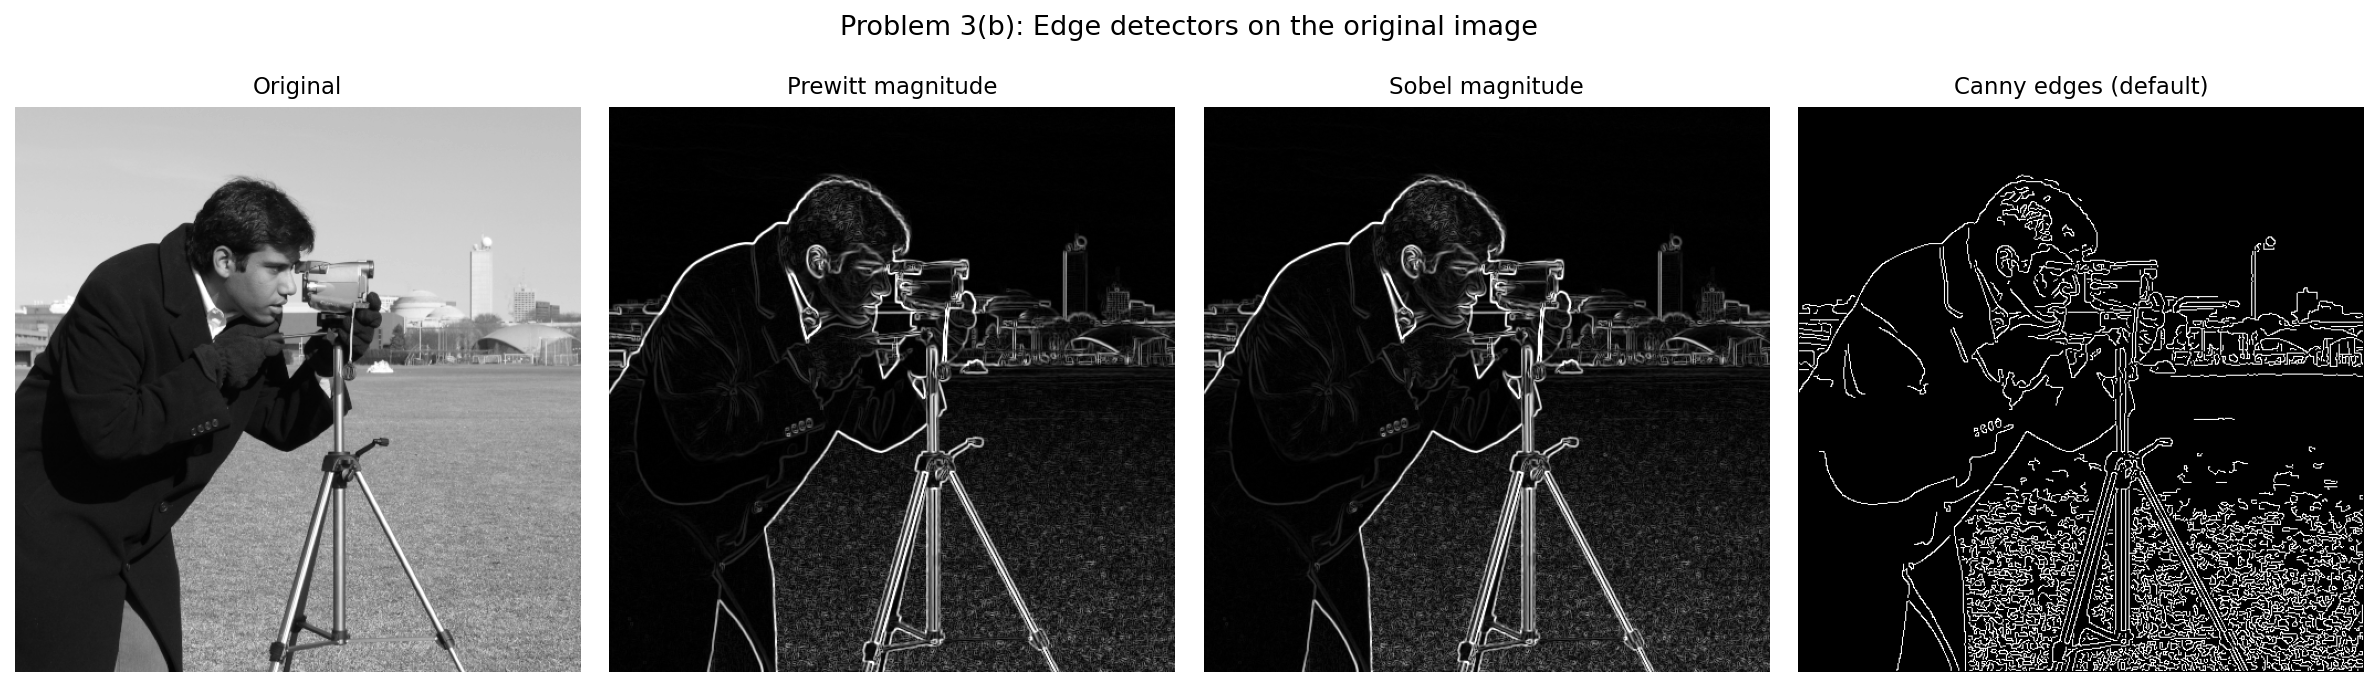
\includegraphics[width=\linewidth]{figures/q3b_clean.png}
\end{figure}

\subsection*{(c)}
\begin{itemize}[leftmargin=*]
\item \textbf{Boundaries:} all three methods find the main boundaries (the man, the camera, the tripod, the skyline). In Prewitt and Sobel, low-contrast edges appear faint. Canny marks every detected edge equally.
\item \textbf{Thickness and continuity:} Prewitt and Sobel edges are thick (2--3 pixels) and vary in brightness. Canny edges are thin (1 pixel) and mostly continuous because of non-maximum suppression and hysteresis.
\item \textbf{Differences:} Prewitt and Sobel look almost identical. Canny gives a binary edge map, but with the default thresholds it also marks a lot of grass texture.
\end{itemize}

\subsection*{(d)}
\begin{figure}[H]\centering
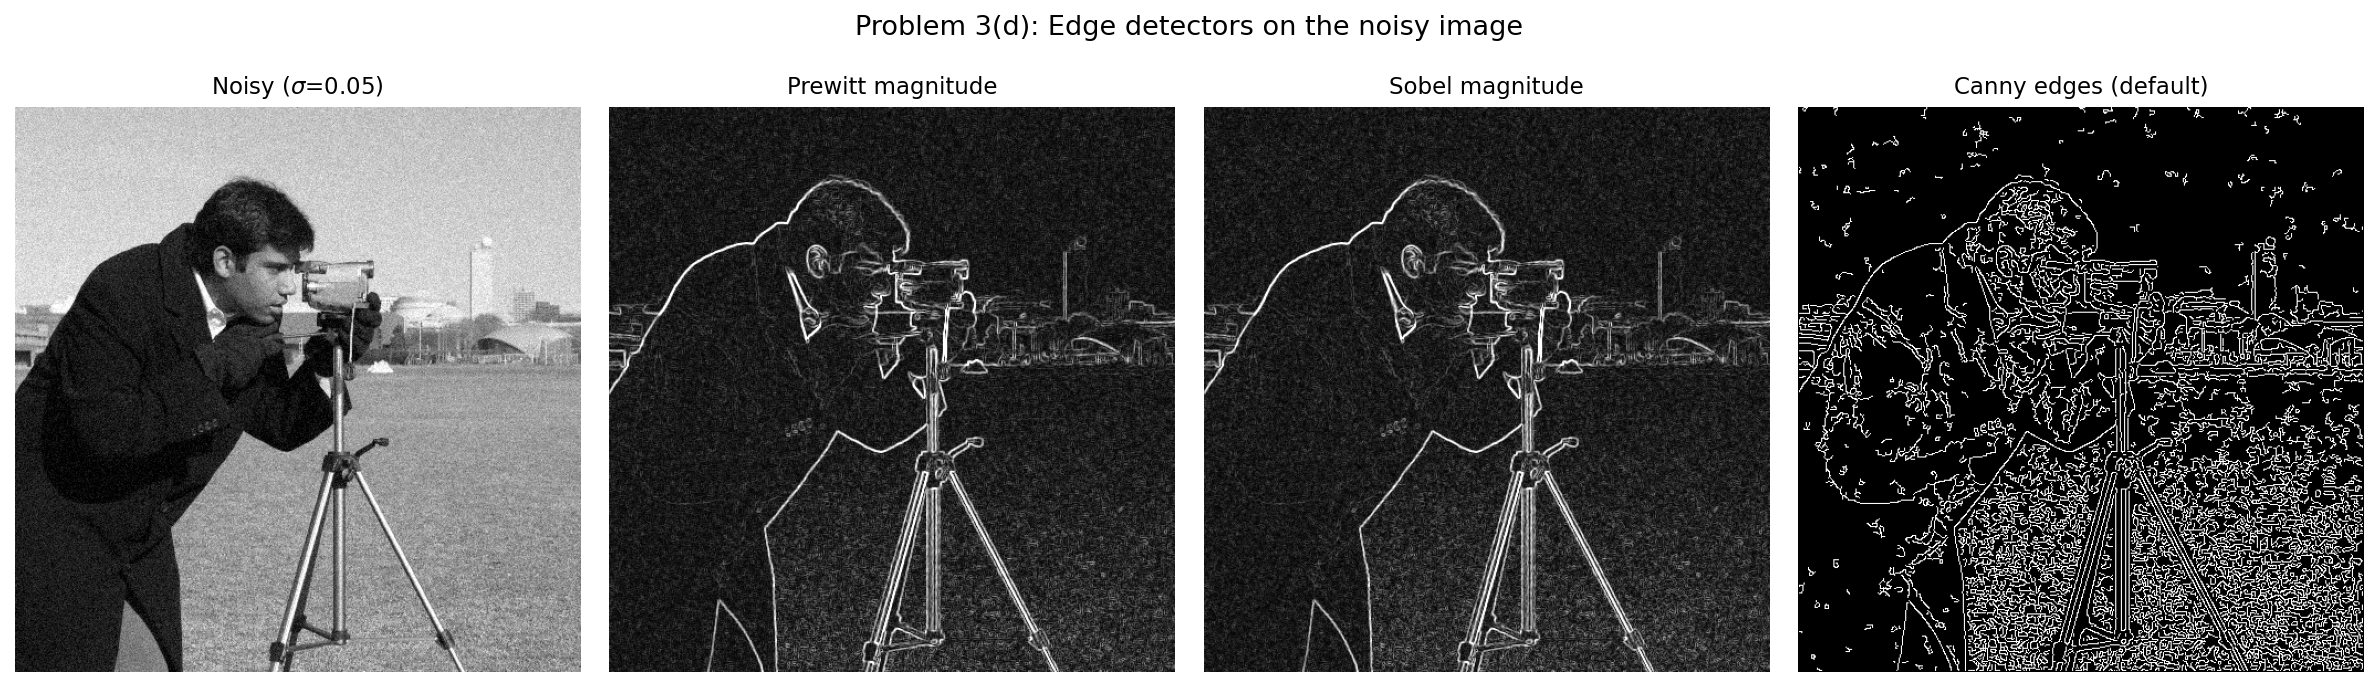
\includegraphics[width=\linewidth]{figures/q3d_noisy.png}
\end{figure}

\begin{table}[H]\centering\small
\begin{tabular}{lcc}\toprule
 & Clean & Noisy\\\midrule
Prewitt: sky response / edge response & 0.0047 & 0.0922\\
Sobel: sky response / edge response & 0.0048 & 0.0948\\
Canny: edge pixels in $100\times100$ sky patch & 0 & 218\\
Canny: clean edges still detected & -- & 94\%\\\bottomrule
\end{tabular}
\end{table}

\subsection*{(e)}
\begin{enumerate}[label=\roman*., leftmargin=*]
\item \textbf{Most sensitive: Prewitt and Sobel} (about equally). The whole background becomes grainy, and the noise level relative to the edges rises about 20$\times$.
\item \textbf{Most robust: Canny.} The main contours stay clean and connected (94\% preserved), and only a few short noise fragments appear.
\item Derivatives amplify high-frequency noise, so the amount of smoothing matters:
  \begin{itemize}
  \item \emph{Prewitt}: a difference combined with a 3-pixel average. Very little smoothing.
  \item \emph{Sobel}: a difference combined with $[1,2,1]$ smoothing. The window is just as small, so it is about equally noisy.
  \item \emph{Canny}: Gaussian smoothing ($\sigma=1$) \emph{before} computing gradients, which greatly reduces the noise. Non-maximum suppression and hysteresis thresholding then remove most of the isolated noise responses.
  \end{itemize}
\end{enumerate}

%=====================================================================
\appendix
\section*{Appendix: Code}
\subsection*{\texttt{hw2\_q2.py}}
\lstinputlisting{hw2_q2.py}
\subsection*{\texttt{hw2\_q3.py}}
\lstinputlisting{hw2_q3.py}

\end{document}
